\documentclass[a4paper, 11pt, oneside]{elsarticle}

\usepackage{listings}
\usepackage{graphicx} \pdfcompresslevel=9
\usepackage[usenames,dvipsnames]{color}
%\usepackage{cite}
\usepackage{setspace}
\usepackage{float}
\usepackage{fancyhdr}
\usepackage{amsmath, amsthm, amssymb}
\usepackage{algorithmic}
\usepackage{algorithm}
\usepackage[utf8]{inputenc}
\usepackage[english]{babel}
\usepackage{url}
\usepackage{appendix}
\usepackage{wrapfig}
\usepackage[hang,small,bf]{caption}
\usepackage{alltt}
\usepackage{hyperref}
\usepackage[margin=3cm]{geometry}
\usepackage{bchart}
\usepackage{framed}
\usepackage{mdframed}
\usepackage{graphicx}
\usepackage{lineno}
\usepackage{bussproofs}
%\usepackage{times}

\lstset{
	language=bash,
	basicstyle=\small\ttfamily,
	keywordstyle=\bfseries,
	commentstyle=\small\color{blue},
	numbers=left,
	numberstyle=\tiny,
	frame=tb,
	columns=fullflexible,
	showstringspaces=false
}

%****************************************************
%********************   MACROS   ********************
%****************************************************

\newcommand{\HRule}{\rule{\linewidth}{0.5mm}}
\setlength{\parindent}{0in}

\newcommand{\itab}[1]{\hspace{0em}\rlap{#1}}
\newcommand{\tab}[1]{\hspace{.2\textwidth}\rlap{#1}}

\newcommand {\ent} {\mathrel{{\scriptstyle\mid\!\sim}}}
\newcommand{\tip}{{\bf T}}
\newcommand{\al}{\mathcal{AL}}
\newcommand{\alc}{\mathcal{ALC}}
\newcommand{\alct}{\mathcal{ALC}+\tip}
\newcommand{\alctmin}{\mathcal{ALC}+\tip_{\mbox{\em min}}}

\newcommand{\hide}[1]{}

\newcommand{\falso} {\bot}
\newcommand{\vero} {\top}
\newcommand{\unione} {\cup}
\newcommand{\intersezione} {\cap}
\newcommand{\unioneq}{\sqcup}
\newcommand{\vuoto} {\emptyset}
\newcommand{\nott} {\lnot}
\newcommand{\tc} {\mid}
\newcommand{\imp} {\rightarrow}
\newcommand{\incluso} {\subseteq}
\newcommand{\appartiene} {\in}
\newcommand{\bbox}{\square}
\newcommand{\diverso} {\neq}
\newcommand{\sqset}{\sqsubseteq}
\newcommand{\subs}{\subseteq}
\newcommand{\mint}{\sqcap}
\newcommand{\mun}{\sqcup}
\newcommand{\sx} {\langle}
\newcommand{\dx} {\rangle}
\newcommand{\modello} {\models}
\newcommand{\perogni} {\forall}
\newcommand{\esiste} {\exists}

\newcommand{\db}{\mathcal{D}(\mbox{\bf B})}
\newcommand{\II} {\mathcal{I}}
\newcommand{\elle} {\mathcal{L}}
\newcommand{\ellet} {\mathcal{L}_{\bf T}}
\newcommand{\emme} {\begin{mathcal}M\end{mathcal}}
\newcommand{\enne} {\begin{mathcal}N\end{mathcal}}
\newcommand{\Gammam}[2]{S^{M}_{#1 \imp #2}}

\newcommand{\nuovoc}{\mathrel{{\mathcal{T}\!\mathcal{AB}}}_{min}^{\mathcal{ALC}+\mbox{\scriptsize $\tip$}}}
\newcommand{\primo}{\mathrel{{\mathcal{T}\!\mathcal{AB}}}_{PH 1}^{\mathcal{ALC}+\mbox{\scriptsize $\tip$}}}
\newcommand{\secondo}{\mathrel{{\mathcal{T}\!\mathcal{AB}}}_{PH 2}^{\mathcal{ALC}+\mbox{\scriptsize $\tip$}}}
\newcommand{\calcolo}{T^{\mathcal{ALC}+\mbox{\scriptsize $\tip$}}}
\newcommand{\trans}[1]{\stackrel{#1}{\longrightarrow}}

%\newcommand{\qed}{{\hspace*{\fill} \rule{2.2mm}{2.2mm}}}

%****************************************************
%******************  ENVIRONMENTS  ******************
%****************************************************

\hide{
\newenvironment{proof}
{\begin{trivlist} \item[] {\bf Proof:}}%
{\qed \end{trivlist}}

\newenvironment{definition}
{\begin{defi} \rm}{\qed \end{defi}}

\newenvironment{proofof}[2]
{\begin{trivlist} \item[] {\bf Proof of #1~\protect{\ref{#2}}.}}%
{\qed \end{trivlist}}


\newenvironment{example}
{\begin{exa} \rm}{\qed \end{exa}}

\newenvironment{remark}
{\begin{rem} \rm}{\end{rem}}
}

\newtheorem{theorem}{Theorem}
\newdefinition{definition}{Definition}
\newdefinition{example}{Example}
\newtheorem{proposition}{Proposition}
\newtheorem{lemma}{Lemma}
%\newproof{proof}{Proof}

\hide{
\newcounter{posu}
\newtheorem{theorem}[posu]{Theorem}
\newtheorem{lemma}[posu]{Lemma}
\newtheorem{corollary}[posu]{Corollary}
\newtheorem{proposition}[posu]{Proposition}
\newtheorem{definition}[posu]{Definition}
\newtheorem{example}[posu]{Example}
\newtheorem{rem}[posu]{Remark}
\newtheorem{proof}[posu]{Proof}
\newtheorem{fact}[posu]{Fact}
}




\begin{document}

%****************************************************
%********************   TITLE   *********************
%****************************************************
\begin{titlepage}
\begin{center}

\begin{figure}[htp]
\centering

\includegraphics[scale=0.25]{img/logo_unito.png}
\label{}
\end{figure}

\textsc{\LARGE Università degli studi di Torino}\\[2cm]
\textsc{\Large Tesi di Laurea Magistrale}\\[2cm]

\HRule \\[0.4cm]
{ \huge \bfseries Thesis title}\\[0.2cm]
\HRule \\[3cm]

% Authors
\begin{flushleft}
{\Large
Candidato:\\[0.5cm]
Luca Violanti}
\end{flushleft}

\end{center}
\end{titlepage}
\newpage

%****************************************************
%*****************  ABSTRACT  ***********************
%****************************************************


%[TODO] scrivere l'abstract
\section*{Abstract}

\newpage

%****************************************************
%********************  TOC  *************************
%****************************************************

\tableofcontents

\newpage

%****************************************************
%***************  INTRODUCTION  *********************
%****************************************************

\section{Introduction}

In this thesis we present the design and implementation of a distributed theorem prover for the non--monotonic description logic $\alctmin$.

Description Logics (DL) are a family of formal knowledge representation languages. They are a decidable fragment of the first-order logic formalism used to provide semantics to representation structures.
DLs are used in artificial intelligence for formal reasoning on the concepts of an application domain. It is of particular importance in providing a logical formalism for ontologies and the Semantic Web. The most notable applications outside information science are in the field of bioinformatics and in the codification of medical knowledge. A DL knowledge base (KB) comprises two components: the TBox, containing the definition of concepts (and possibly roles) and a specification of inclusion relations among them, and the ABox containing instances of concepts and roles. Since the very objective of the TBox is to build a taxonomy of concepts, the need of representing prototypical properties and of reasoning about defeasible inheritance of such properties naturally arise. The traditional approach is to handle defeasible inheritance by integrating some kind of non--monotonic extension of DLs.

In chapter \ref{dl} we introduce the Description Logics and briefly describe some proposals for non--monotonic extensions, while in chapter \ref{dlt} we describe the non--monotonic logic $alctmin$.\\

Our implementation is based on the tableaux proof method that is a mechanism that allows to demonstrate the validity of a formula in a given logical system.
The tableaux calculus allows us to conclude that a formula is valid (or not) just by applying the tableaux computation rules, i.e., without appealing to the semantics.
Proof methods can be implemented in many different programming languages, but logic programming languages offer a better solution since in this paradigm we make use of mathematical logic for computer programming.
Logic programming in the first and wider sense gave rise to a large number of implementations. Foster and Elcock’s Absys (1969), was probably the first language to be explicitly developed as an assertional programming language. Logic programming in the narrower sense can be traced back to debates in the late 1960s and early 1970s about declarative versus procedural representations of knowledge in Artificial Intelligence.

In chapter \ref{tab} we introduce the tableaux calculus for $\alctmin$, which is at the base of our theorem prover\ref{arch}.\\

Since our work is an expansion of a previous theorem prover called PreDeLo, chapter \ref{predelo} is dedicated to its description. In chapter \ref{bg} we 

In chapter 


\ref{arch}\\

In our implementation we used SICStus Prolog and for this reason we dedicate Chapter 2 to analyse its fundamental concepts.
The Prolog engine of our application was the first component to be developed. In Chapter 5 we will describe in details the implementations and their structures explaining what considerations driven our choices.
The theorem prover’s functionalities are accessible through a graphical user interface (GUI) that has been developed in the Java programming language.
These functionalities are described in detail in Chapter 6.
We will also provide a brief explanation of how Java and Prolog are interconnected and work together.
Finally, we will describe what are the possible future improvements.
Our main idea is to deploy the theorem prover in a distributed environment.
Since we often have to deal with high complexity calculi, grid computing could offer a solution for distributing such complexity on different computing resources.
Different approaches for distributed Prolog implementations already exists and they are described in literature.
A general description of our design idea will be given in Chapter 7.


%[TODO] completare introduzione

%\chapter{Why}
%\chapter{What}
%\chapter{Logics}
%\chapter{The problem}
%\chapter{Automated reasoning}
%\chapter{State of the art}

\newpage


%****************************************************
%*********************  DL  *************************
%****************************************************

\section{Description Logics}\label{dl}

Description Logics are decidable fragments of the first-order logic formalism used to provide semantics to representation structures like frames and networks.
Each fragment has different features, leading to computational problems of variable complexity: the use of a more simple language (low computational complexity) rather than a more expressive one (high computational complexity) depends on how complex we want the world description to be.


\begin{figure}[htp]
\centering
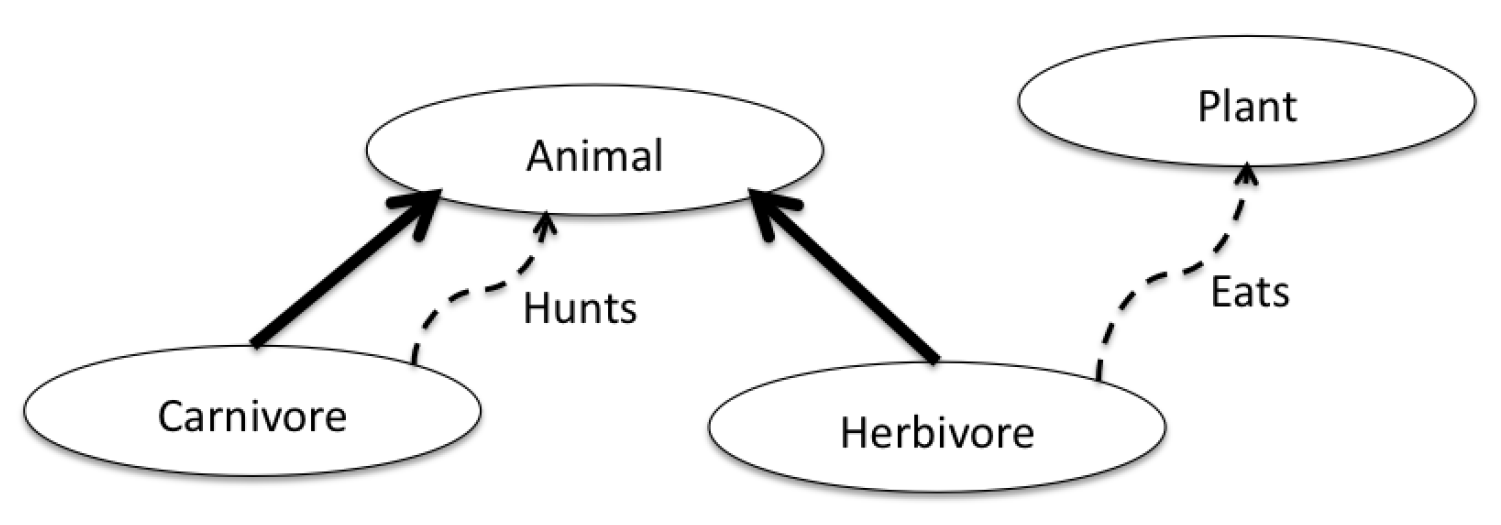
\includegraphics[scale=.33]{img/relationship_network.png}
\caption{An example of network, showing relationships between concepts.}
\label{rel_net}
\end{figure}

Typically, nodes are used to characterize concepts, i.e., sets of individuals, and links are used to characterize relationships among them.
Concepts can have simple properties, which are typically attached to the corresponding nodes.
It is rather simple to make a correspondence between network structures and Description Logics because the latter are equipped with unary predicates representing sets of individuals, binary predicates representing relationships among them and a mechanism of inclusion statements to express concept properties.
Indeed, we can represent concept properties with the inclusion statement $Carnivore \sqsubseteq Animal$ and we can express the following facts about an individual $lion$: 

\begin{itemize}
	\item $Carnivore(lion)$
	\item $Hunts(lion, zebra)$
	\item $Herbivore(elephant)$
	\item $Eats(elephant, grass)$
\end{itemize}

It is also possible to use intersection concepts with the syntax $Carnivore \sqcap Plant$ to select individuals which belong to both $Carnivore$ and $Plant$.

\newpage

\subsection{Application domains}
Description Logics are used in the implementation of many systems that demonstrate their practical effectiveness. Some of these systems have found their way into production use, despite the fact that there was no real commercial platform that could be used for developing them.\\

\textbf{Software engineering.} Software Engineering was one of the first application domains for Description Logics. The basic idea was to use a Description Logic to implement a Software Information System, i.e. a system that would support the software developer by helping him in finding out information about a large software system.\\

\textbf{Configuration management.} One very successful domain for knowledge-based applications built using Description Logics is configuration management, which includes applications that support the design of complex systems created by combining multiple components.
The main goal of this discipline is finding a proper set of components that can be suitably connected in order to implement a system that meets a given specification.
For example, choosing computer components in order to build a home PC is a relatively simple configuration task.
When the number, the type, and the connectivity of the components grow, the configuration task can become rather complex.
In particular, computer configuration has been among the application fields of the first Expert Systems and can thus be viewed as a standard application domain for knowledgebased systems.
Configuration tasks arise in many industrial domains, such as telecommunications, the automotive industry, building construction, etc.
DL-based knowledge representation systems meet the requirements for the development of configuration applications.
In particular, they enable the object-oriented modelling of system components, which combines powerfully with the ability to reason from incomplete specifications and to automatically detect inconsistencies.
Using Description Logics one can exploit the ability to classify the components and organize them within a taxonomy.\\

\textbf{Medicine.} Medicine is also a domain where Expert Systems have been developed since the 1980’s, in particular in the field of decision support for medical diagnosis. One focus has been on the construction and maintenance of very large ontologies of medical knowledge, the subject of some large government initiatives.
In order to cope with the scalability of the knowledge base, the DL language adopted in these applications is often limited to a few basic constructs and the knowledge base turns out to be rather shallow, that is to say the taxonomy does not have very many levels of sub-concepts below the top concepts.\\

\textbf{Data mining.} Description Logics have also been used in data mining applications, where their inferences can help the process of analysing large amounts of data.
In this kind of application, DL structures can represent views, and DL systems can be used to store and classify such views. The classification mechanism can help in discovering interesting classes of items in the data
\cite{Nardi:2003:IDL:885746.885748}.

\newpage

\subsection{Basic Description Logics}
As the name Description Logics indicates, one of the characteristics of these languages is that they are equipped with a formal, logic-based semantics.
Another distinguished feature is the emphasis on reasoning as a central service: reasoning allows one to infer implicitly represented knowledge from the knowledge that is explicitly contained in the knowledge base.
Description Logics support inference patterns that occur in many applications of intelligent information processing systems, and which are also used by humans to structure and understand the world: classification of concepts and individuals.
Classification of concepts determines subconcept/superconcept relationships (called subsumption relationships in DL) between the concepts of a given terminology, and thus allows one to structure the terminology in the form of a subsumption hierarchy.
Classification of individuals (or objects) determines whether a given individual is always an instance of a certain concept (i.e., whether this instance relationship is implied by the description of the individual and the definition of the concept).
It thus provides useful information on the properties of an individual.
Moreover, instance relationships may trigger the application of rules that insert additional facts into the knowledge base.
The implementation of reasoning services requires building procedures that should always terminate, both for positive and for negative answers, but also complexity needs to be taken into consideration.
Decidability and complexity of the inference problems depend on the expressive power of the DL at hand.
On the one hand, very expressive DLs are likely to have inference problems of high complexity.
On the other hand, very weak DLs (with efficient reasoning procedures) may not be sufficiently expressive to represent the important concepts of a given application.
Investigating this trade-off between the expressivity of DLs and the complexity of their reasoning problems is one of the most important issues in DL research
\cite{Baader:2003:BDL:885746.885749}.


\newpage

\subsection{The basic description language $\al$}
A knowledge representation system based on Description Logics provides facilities to set up knowledge bases, to reason about their content, and to manipulate them.
A knowledge base (KB) comprises two components, the TBox and the ABox.
The TBox introduces the terminology, i.e., the vocabulary of an application domain, while the ABox contains assertions about named individuals in terms of this vocabulary.
The vocabulary consists of concepts, which denote sets of individuals, and roles, which denote binary relationships between individuals.
Elementary descriptions are atomic concepts and atomic roles.
Complex descriptions can be built from them inductively with concept constructors.
In abstract notation, we use the letters $A$ and $B$ for atomic concepts, the letter $R$ for atomic roles, and the letters $C$ and $D$ for concept descriptions.
In the sequel we present the language $\al$ that has been introduced in \cite{Schmidt-SchaubB:1991:ACD:114341.114342} as a minimal language that is of practical interest. The other languages of this family are extensions of $\al$.

Concept descriptions in $\al$ are formed according to the following syntax rule:\\

\begin{itemize}
\item[] $C, D \imp$
\item[] \itab{$A \tc$} \tab{(atomic concept)}
\item[] \itab{$\vero \tc$} \tab{(top concept - most general)}
\item[] \itab{$\falso \tc$} \tab{(bottom concept - most specific)}
\item[] \itab{$\neg A \tc$} \tab{(atomic negation)}
\item[] \itab{$C \mint D \tc$} \tab{(intersection)}
\item[] \itab{$\forall R.C \tc$} \tab{(value restriction)}
\item[] \itab{$\exists R.\vero $} \tab{(limited existential quantification)}
\end{itemize}


In order to define a formal semantics of $\al$-concepts we consider interpretations $\II$ that consist of a non-empty set $\Delta$ (the domain of the interpretation) and an interpretation function, which assigns to every atomic concept $A$ a set $A^{\II} \subseteq \Delta^{\II}$ and to every atomic role R a binary relation $R^{\II} \subseteq \Delta^{\II} \times \Delta^{\II}$. The
interpretation function is extended to concept descriptions by the following
inductive definitions:

\begin{itemize}
\item[] \itab{$\vero^{\II} = \Delta^{\II}$}
\item[] \itab{$(\neg A)^{\II} = \Delta^{\II} $\textbackslash $A^{\II}$}
\item[] \itab{$(C \mint D)^{\II} = C^{\II} \mint D^{\II}$}
\item[] \itab{$(\forall R.C)^{\II} = \left\{x \in \Delta \tc \perogni y.(x, y)\in R^{\II} \imp y \in C^{\II} \right\}$}
\item[] \itab{$(\exists R.\vero)^{\II} = \left\{x \in \Delta \tc \esiste y.(x, y)\in R^{\II} \right\}$}
\end{itemize}

We say that two concepts $C$, $D$ are equivalent, and write $C = D$, if $C^{\II} = D^{\II}$ for all interpretations $\II$
\cite{Baader:2003:BDL:885746.885749}.

\subsection{Complex concept negation: $\alc$}
A basic extension of $\al$ is the negation of an arbitrary concept:
\begin{itemize}
\item[] \itab{$\neg C$} \tab{(concept negation)}
\end{itemize}

whose semantics is:
\begin{itemize}
\item[] \itab{$(\neg C)^{\II} = \Delta^{\II} $\textbackslash $C^{\II}$}
\end{itemize}
\cite{obitko}


\subsection{Non--monotonic reasoning and the operator $\tip$}
Since the very objective of the TBox is to build a taxonomy of concepts, the need of representing prototypical properties and of reasoning about defeasible inheritance of such properties easily arises.
The traditional approach is to handle defeasible inheritance by integrating some kind of non--monotonic reasoning mechanism.
This has led to study non--monotonic extensions of DLs \cite{baader95a, baader95b, bonattilutzwolterkr06, casinistraccia2010, donini98, donini2002, eiter2004, straccia93}.
However, finding a suitable non--monotonic extension for inheritance reasoning with exceptions is far from obvious.
To give a brief account, \cite{baader95a} proposes the extension of DL with Reiter's default logic.
However, the same authors have pointed out that this integration may lead to both semantical and computational difficulties.
Indeed, the unsatisfactory treatment of open defaults via Skolemization may lead to an undecidable default consequence relation. For this reason, \cite{baader95a} proposes a restricted semantics for open default theories, in which default rules are only applied to individuals explicitly mentioned in the ABox.
Furthermore, Reiter's default logic does not provide a direct way of modeling inheritance with exceptions.
This has motivated the study of extensions of DLs with prioritized defaults
\cite{straccia93,baader95b}.
A more general approach is undertaken in \cite{donini2002}, where it is proposed an extension of DL with two epistemic operators. This extension allows to encode Reiter's default logic as well as to express epistemic concepts and procedural rules.
In \cite{bonattilutz} the authors propose an extension of DL with circumscription. One of the motivating applications of circumscription is indeed to express prototypical properties with exceptions, and this is done by introducing ``abnormality'' predicates, whose extension is minimized.
The authors provide decidability and complexity results based on theoretical analysis.
A tableau calculus for circumscriptive $\mathcal{ALCO}$ is presented in \cite{hitzlertableau}.

In \cite{casinistraccia2010,stracciaijcai2011} a non--monotonic extension of $\mathcal{ALC}$  based on the application of Lehmann and Magidor's \emph{rational closure} \cite{whatdoes} to $\mathcal{ALC}$ is proposed. The approach is based on the introduction of a consequence relation $\ent$ among concepts and of a consequence relation $\Vdash$ among an unfoldable KB and assertions. The authors show that such consequence relations are \emph{rational}. It is also shown that such relations inherit the same computational complexity of the underlying DL.

Recent works discuss the combination of open and closed world reasoning in DLs. In particular, formalisms have been defined for combining DLs with logic programming rules (see, for instance, \cite{eiter2004} and \cite{rosatiacm}). A grounded circumscription approach for DLs with local closed world capabilities has been defined in \cite{hitzlerdl}.

\newpage

A non--monotonic extension should have the following characteristics:

\begin{enumerate}
\item The (non--monotonic) extension must have a clear semantics and should be based on the same semantics as the underlying monotonic DL.
\item The extension should allow to specify prototypical properties in a natural and direct way.
\item The extension must be decidable, if  so is the underlying monotonic DL, and standard proof methods for monotonic DL should be generalized to it.
\end{enumerate}

%%TODO  controllare bene questa parte

Before entering the technical details, let us sketch how the pre--existent work makes use of the typicality operator $\tip$ for inference. The KB is comprised of the standard TBox and ABox, with the addition of a set of assertions of the form $\tip(C)\sqsubseteq D$, where $D$ is a concept not mentioning $\tip$.

For instance, let the TBox contain:

\begin{quote}
$\tip (\mathit{Student}) \sqset \mathit{\neg IncomeTaxPayer}$\\
$\tip (\mathit{Student} \mint \mathit{Worker})  \sqset \mathit{IncomeTaxPayer}$\\
$\tip (\mathit{Student} \mint \mathit{Worker} \mint \mathit{Erasmus})  \sqset \mathit{\neg IncomeTaxPayer}$
\end{quote}


\noindent corresponding to the assertions: typical students don't have to pay income taxes, whereas if a student is also a worker, typically he will pay income taxes; if an Erasmus Programme student is also a worker, he does not have to pay income taxes.
Suppose  further that the ABox contains alternatively one of the following facts:

\begin{quote}
1. $\mathit{Student}(\mathit{luca})$ \\
2. $\mathit{Student}(\mathit{antonio}), \mathit{Worker}(\mathit{antonio})$ \\
3. $\mathit{Student}(\mathit{marco}), \mathit{Worker}(\mathit{marco}), Erasmus(\mathit{marco})$
\end{quote}


\noindent From the different combinations of TBox and one of the above ABox assertions (either $1$ or $2$ or $3$), we can infer the expected (defeasible) conclusions. These are, respectively:

\begin{quote}
1. $\mathit{\neg IncomeTaxPayer}(\mathit{luca})$\\
2. $\mathit{IncomeTaxPayer}(\mathit{antonio})$ \\
3. $\mathit{\neg IncomeTaxPayer}(\mathit{marco})$
\end{quote}

\noindent Moreover, we would also like to infer (defeasible) properties of individuals
implicitly introduced by existential restrictions, for instance,
if the ABox contains

\begin{quote}
$\exists \mathit{HasChild}.\mathit{Student(grazia)}$
\end{quote}

\noindent we would like to infer that:
\begin{quote}
$\exists \mathit{HasChild.\neg IncomeTaxPayer(grazia)}$
\end{quote}

\noindent Finally, adding irrelevant information should not affect the conclusions. From the TBox above, one should be able to infer as well

\begin{quote}
$\tip (\mathit{Student} \mint \mathit{Tall}) \sqset \mathit{\neg IncomeTaxPayer}$\\
$\tip (\mathit{Student} \mint \mathit{Worker} \mint \mathit{Tall})  \sqset \mathit{IncomeTaxPayer}$ \\
$\tip (\mathit{Student} \mint Worker \mint Erasmus \mint \mathit{Tall})  \sqset \mathit{\neg IncomeTaxPayer}$
\end{quote}

\noindent as  $\mathit{Tall}$ is irrelevant with respect to paying income taxes or not. For the same reason, the conclusion about $\mathit{luca}$ being an instance of $\neg IncomeTaxPayer$ or not should not be influenced by adding $\mathit{Tall}(\mathit{luca})$ to the ABox.\\

Hereinafter we introduce a non--monotonic extension for defeasible reasoning in description logics, called $\alctmin$, which is an extension of $\alct$.

%%TODO fine parte da controllare

\newpage

%****************************************************
%******************  DL + T  ************************
%****************************************************

\section{Description Logics for typicality}\label{dlt}

\subsection{The logic $\alct$}\label{alct}


In this section, we recall the original $\alct$, which is an extension of $\alc$ by a typicality operator $\tip$ introduced in \cite{FI09}. Given an alphabet of concept names $\mathcal{C}$, of role names $\mathcal{R}$, and of individual constants $\mathcal{O}$, the language $\elle$ of the logic $\alct$ is defined by distinguishing \emph{concepts} and \emph{extended concepts} as follows:

\begin{itemize}
\item (Concepts)
  \begin{itemize}
     \item $A \in \mathcal{C}$, $\vero$ and $\bot$ are \emph{concepts} of
$\elle$;
    \item if $C, D \in \elle$ and $R \in \mathcal{R}$, then $C
\sqcap D, C \sqcup D, \neg C, \forall R.C, \exists R.C$ are
\emph{concepts} of $\elle$
  \end{itemize}
\item (Extended concepts)
    \begin{itemize}
       \item if $C$ is a
concept of $\elle$, then $C$ and $\tip(C)$ are \emph{extended concepts} of $\elle$
     \item boolean combinations of extended concepts are extended
concepts of $\elle$.
    \end{itemize}
\end{itemize}

\noindent  A knowledge base is a pair (TBox, ABox). TBox contains subsumptions $C \sqsubseteq D$, where $C \in \elle$ is an extended concept of the form either $C'$ or $\tip(C')$, and $C', D \in \elle$ are concepts.
ABox contains expressions of the form $C(a)$ and $aRb$ where $C \in \elle$ is an extended concept, $R \in \mathcal{R}$, and $a, b \in \mathcal{O}$.



In order to provide a semantics to the operator $\tip$, we extend the definition of a model used in ``standard'' terminological logic $\alc$:

\begin{definition}[Semantics of $\tip$ with selection function]\label{Semantics with f_tip} A model is any structure $\langle \Delta, I, f_\tip \rangle$ where:

\begin{itemize}
\item $\Delta$ is the domain, whose elements are denoted with $x, y, z, \dots$;
\item $I$ is the extension function that maps each extended concept $C$ to $C^I \subseteq \Delta$, and each role $R$ to a $R^I \subseteq \Delta \times \Delta$.
$I$ assigns to each atomic concept $A \in \mathcal{C}$ a set $A^I \subseteq \Delta$ and it is extended to arbitrary extended concepts as follows:

\begin{itemize}
  \item $\top^I=\Delta$
  \item $\bot^I=\vuoto$
  \item $(\nott C)^I=\Delta \backslash C^I$
  \item $(C \sqcap D)^I=C^I \cap D^I$
  \item $(C \sqcup D)^I=C^I \cup D^I$
  \item $(\forall R.C)^I=\{x \in \Delta \tc \forall y. (x,y) \in R^I \imp y \in C^I\}$
  \item $(\exists R.C)^I=\{x \in \Delta \tc \exists y.(x,y) \in R^I \ \mbox{and} \ y \in C^I\}$
  \item $(\tip(C))^I = f_\tip(C^I)$
\end{itemize}


\item Given $S \subseteq \Delta$, $f_\tip$ is a function $f_\tip : Pow(\Delta) \rightarrow Pow(\Delta)$ satisfying the following properties:

\begin{itemize}
\item $(f_\tip-1)$ $f_\tip(S) \subseteq S$;
\item $(f_\tip-2)$ if $S \neq \emptyset$, then also $f_\tip(S)
\neq \emptyset$;
\item $(f_\tip-3)$ if $f_\tip(S) \subseteq R$, then $f_\tip(S) = f_\tip(S \cap R)$;
\item $(f_\tip-4)$ $f_\tip(\bigcup S_i ) \subseteq \bigcup f_\tip(S_i)$;
\item $(f_\tip-5)$ $\bigcap f_\tip(S_i) \subseteq  f_\tip(\bigcup S_i)$.
\end{itemize}

\end{itemize}

\end{definition}

\noindent Intuitively, given the extension of some concept $C$, the selection function $f_\tip$ selects  the {\em typical} instances of $C$.
($f_\tip-1$) requests that typical elements of $S$ belong to $S$.
($f_\tip-2$) requests that if there are elements in $S$, then there are also {\em typical} such elements.
The following properties constrain the behaviour of $f_\tip$ with respect to $\cap$ and $\cup$ in such a way that they do not entail monotonicity.
According to ($f_\tip-3$), if the typical elements of $S$ are in $R$, then they coincide with the typical elements of $S \cap R$, thus expressing a weak form of monotonicity (namely, {\em cautious monotonicity}).
($f_\tip-4$) corresponds to one direction of the equivalence $f_\tip(\bigcup S_i) = \bigcup f_\tip(S_i)$, so that it does not entail monotonicity.
Similar considerations apply to the equation $f_\tip(\bigcap S_i) = \bigcap f_\tip(S_i)$, of which only the inclusion $\bigcap f_\tip(S_i) \incluso f_\tip(\bigcap S_i)$ holds. ($f_\tip-5$) is a further constraint on the behavior of $f_\tip$ with respect to arbitrary unions and intersections; it would be derivable if $f_\tip$ were monotonic.

In \cite{FI09}, it is shown that one can give an equivalent, alternative semantics for $\tip$ based on a \emph{preference relation} semantics rather than on a selection function semantics.
The idea is that there is a global, irreflexive and transitive relation among individuals and that the typical members of a concept $C$ (i.e., those selected by $f_\tip(C^I)$) are the minimal elements of $C$ with respect to this relation.
Observe that this notion is \emph{global}, that is to say, it does not compare individuals with respect to a specific concept.
For this reason,  we cannot express the fact that $y$ is more typical than $x$ with respect to concept $C$, whereas $x$ is more typical than $y$ with respect to another concept $D$.
All what we can say is that either $x$ is incomparable with $y$ or $x$ is more typical than $y$ or $y$ is more typical than $x$.
In this framework, an element $x \in \Delta$ is a {\em typical instance} of some concept $C$ if $x \in C^I$ and there is no $C$-element in $\Delta$ {\em more typical} than $x$.
The typicality preference relation is partial since it is not always possible to establish given two element which one of the two is more typical.
Following KLM, the preference relation also satisfies a \emph{Smoothness Condition}, which is related to the well known \emph{Limit Assumption} in Conditional Logics \cite{Nute80}
\footnote{More precisely, the Limit Assumption entails the Smoothness Condition (i.e. that there are no infinite $<$ descending chains). Both properties come for free in finite models.};
this condition ensures that, if the extension $C^I$ of a concept $C$ is not empty, then there is at least one \emph{minimal} element of $C^I$.
This is stated in a rigorous manner in the following definition:

\begin{definition}\label{Definition of $<$} Given an irreflexive and transitive relation  $<$ over a domain $\Delta$, called \emph{preference relation}, for all $S \subseteq \Delta$, we define

$Min_<(S)= \{x \in S \tc \nexists y \in S \ \mbox{s.t.} \ y < x \}$

\noindent We say that $<$ satisfies the {\em Smoothness Condition} if for all $S \subseteq \Delta$, for all $x \in S$, either $x \in Min_<(S)$ or $\exists y \in  Min_<(S)$ such that $y < x$.
\end{definition}

\noindent The following representation theorem is proved in \cite{FI09}:

\begin{theorem}[Theorem 2.1 in \cite{FI09}]\label{rtrt} Given any model $\langle \Delta, I, f_\tip
\rangle$, $f_\tip$ satisfies postulates $(f_\tip-1)$ to $(f_\tip-5)$ above iff there exists  an irreflexive and transitive relation $<$ on $\Delta$, satisfying the Smoothness Condition, such that for all $S \subseteq \Delta$, $f_\tip(S) = Min_<(S)$.
\end{theorem}


\noindent Having the above Representation Theorem, from now on, we will refer to the following semantics:

\begin{definition}[Semantics of $\alct$]\label{Semantics of T} A model $\emme$ of $\alct$ is any structure $$\langle \Delta, I, < \rangle$$ where:

\begin{itemize}

\item $\Delta$ is the domain;

\item $<$ is an irreflexive and transitive relation over $\Delta$ satisfying the Smoothness Condition (Definition \ref{Definition of $<$})

\item $I$ is the extension function that maps each  extended concept $C$ to $C^I \subseteq \Delta$, and each role $R$ to a $R^I \subseteq \Delta \times \Delta$.
$I$ assigns to each atomic concept $A \in \mathcal{C}$ a set $A^I \subseteq \Delta$.
Furthermore, $I$ is extended as in Definition \ref{Semantics with f_tip} with the exception of $(\tip(C))^I$, which is defined as $$(\tip(C))^I = Min_<(C^I).$$
\end{itemize}

\end{definition}

\noindent Let us now introduce the notion of satisfiability of an $\alct$ knowledge base.
In order to define the semantics of the assertions of the ABox, we  extend the function $I$ to individual constants;  we assign to each individual constant $a \in \mathcal{O}$ a \emph{distinct} domain element $a^I \in \Delta$, that is to say we enforce the \emph{unique name assumption}.
As usual, the adoption of the  unique name assumption greatly simplifies reasoning about prototypical properties of individuals denoted by different individual constants.
Considering the example of department staff having lunches, if (in addition to the TBox) the ABox only contains the following facts about Greg and Sara:

\begin{quote}
$\mathit{DepartmentMember}(\mathit{greg})$ \\
$\mathit{DepartmentMember}(\mathit{sara}), \mathit{TemporaryWorker}(\mathit{sara})$
\end{quote}

\noindent we would like to infer that Greg takes his lunches at the restaurant, whereas Sara does not; but without the unique name hypothesis, we cannot get this conclusion since Greg and Sara might be the same individual.
To perform useful reasoning we would need to  extend the language with equality and make a case analysis according to possible identities of individuals. While this is technically possible, we prefer to keep the things simple here by adopting the unique name assumption.

\begin{definition}[Model satisfying a Knowledge Base]\label{Def-ModelSatTBox-ABox} Consider a model $\emme$, as defined in Definition \ref{Semantics of T}.
We extend $I$ so that it assigns to each individual constant $a$ of $\mathcal{O}$ an element $a^I \in \Delta$,  and $I$ satisfies the unique name assumption. Given a KB (TBox,ABox), we say that:

\begin{itemize}
\item $\emme$  satisfies TBox iff  for all  inclusions $C \sqsubseteq D$  in TBox, $C^I \subseteq D^I$.
\item $\emme$ satisfies ABox  iff:
(i) for all $C(a)$  in ABox, we have that $a^I \in C^I$,
(ii) for all $aRb$ in ABox, we have that $(a^I,b^I) \in R^I$.
\end{itemize}

\noindent $\emme$ satisfies a knowledge base if it satisfies both its TBox and its ABox.
Last, a query $F$  is  entailed by KB in $\alct$ if it holds in all models satisfying \emph{KB}.
In this case we write \emph{KB} $\models_{\alct} F$.
\end{definition}


\noindent Notice that the meaning of $\tip$ can be split into two parts: for any $x$ of the domain $\Delta$,  $x \in (\tip(C))^I$ just in case (i) $x \in C^I$, and (ii) there is no $y \in C^I$ such that $y < x$.
As already mentioned in the Introduction, in order to isolate the second part of the meaning of $\tip$ (for the purpose of the calculus that we will present in Section \ref{calcolo}), we introduce a new modality $\bbox$.
The basic idea is simply to interpret the preference relation $<$ as an accessibility relation.
By the Smoothness Condition, it turns out that $\bbox$ has the properties as in G\"odel-L\"ob modal logic of provability G.
The Smoothness Condition ensures that typical elements of $C^I$ exist whenever $C^I \diverso \vuoto$, by avoiding infinitely descending chains of elements.
This condition therefore corresponds to the finite-chain condition on the accessibility relation (as in G).
The interpretation of $\bbox$ in $\emme$ is as follows:

\begin{definition}\label{def-box}
Given a model $\emme$ as in Definition \ref{Semantics of T}, we extend the definition of $I$ with the following clause:
\begin{center}
	$(\bbox C)^I = \{x \in \Delta \tc $  for every $y \appartiene \Delta$, if $y < x$ then $y \in C^I \}$
\end{center}
\end{definition}


\noindent It is easy to observe that $x$ is a typical instance  of $C$ if and only if it is an instance of $C$ and $\bbox \nott C$, that is to say:

\begin{proposition}\label{Relation between T an box}
Given a model $\emme$ as in Definition \ref{Semantics of T}, given a concept $C$ and an element $x \in \Delta$, we have that $$x \in (\tip(C))^I \ \mbox{iff} \  x \in (C \sqcap \bbox \neg C)^I$$
\end{proposition}

\noindent
Since we only use $\bbox$ to capture the meaning of $\tip$, in the following we will always use the modality $\bbox$ followed by a negated concept, as in $\bbox \neg C$.

The Smoothness condition, together with the transitivity of $<$, ensures the following Lemma:

\begin{lemma}\label{ssc}
Given an $\alct$ model as in Definition \ref{Semantics of T}, an extended concept $C$, and an element $x \in \Delta$, if there exists $y < x$ such that $y \in C^I$, then either $y \in Min_<(C^I)$ or there is $z<x$ such that $z \in Min_<(C^I)$.
\end{lemma}

%[TODO] Aggiungere riferimento alla dimostrazione


Last, we state a theorem which will be used in the following:

\begin{theorem}[Finite model property of $\alct$]\label{fmpALCT}
The logic $\alct$ has the finite model property.
\end{theorem}

%[TODO] Aggiungere riferimento alla dimostrazione



\subsection{The logic $\alctmin$}\label{alctmin}

As mentioned in the Introduction, the logic $\alct$ presented in \cite{FI09} allows  to reason about typicality.
As a difference with respect to standard $\alc$, in $\alct$ we can consistently express, for instance, the fact that three different concepts, like {\em Department member}, {\em Temporary Department Member} and {\em Temporary Department member having restaurant tickets}, have a different status with respect to {\em Have lunch at a restaurant}. This can be consistently expressed by including in a knowledge base the three formulas:

\begin{quote}
$\tip (\mathit{DepartmentMember}) \sqset \mathit{LunchAtRestaurant}$\\
$\tip (\mathit{DepartmentMember} \mint \mathit{TemporaryResearcher})  \sqset \nott \mathit{LunchAtRestaurant}$\\
$\tip (\mathit{DepartmentMember} \mint \mathit{TemporaryResearcher} \mint \exists \mathit{Owns}.\mathit{RestaurantTicket})  \sqset \mathit{LunchAtRestaurant}$
\end{quote}

\noindent Assume that $\mathit{greg}$ is an instance of the concept
$\mathit{DepartmentMember} \sqcap \mathit{TemporaryResearcher} \sqcap \exists \mathit{Owns}.\mathit{RestaurantTicket}$. What can we conclude about
$\mathit{\mathit{greg}}$? We have already mentioned that if the ABox explicitly points out that $\mathit{greg}$ is a {\em typical} instance of the  concept, and it contains the assertion that:

$(*)  \ \tip(\mathit{DepartmentMember} \sqcap \mathit{TemporaryResearcher} \sqcap \exists \mathit{Owns}.\mathit{RestaurantTicket})(\mathit{greg}),$


\noindent then, in $\alct$, we can conclude that

$\mathit{LunchAtRestaurant(\mathit{greg})}.$

\noindent However, if (*) is replaced by the weaker $(**)  \ (\mathit{DepartmentMember} \sqcap \mathit{TemporaryResearcher} \sqcap \exists \mathit{Owns}.
\mathit{RestaurantTicket})(\mathit{greg}),$ in which there is no information about the typicality of $\mathit{greg}$, in $\alct$ we can no longer draw this conclusion, and indeed we cannot make any inference about whether $\mathit{greg}$ spends its lunch time at a restaurant or not. The limitation here lies in the fact that $\alct$ is {\em monotonic}, whereas we would like to make a non--monotonic inference.
Indeed, we would like to non--monotonically assume, in the absence of information to the contrary, that $\mathit{greg}$ is a typical instance of the concept.
In general, we would like to infer that individuals are typical instances of the concepts they belong to, if this is consistent with the KB.

As a difference with respect to $\alct$, $\alctmin$ is {\em non--monotonic}, and it allows to make this kind of inference.
Indeed, in $\alctmin$ if (**) is all the information about $\mathit{greg}$ present in the ABox, we can derive that $\mathit{greg}$ is a typical instance of the concept, and from the inclusions above we conclude that $\mathit{LunchAtRestaurant(\mathit{greg})}.$
We have already mentioned that we obtain this non--monotonic behaviour by restricting our attention to the  minimal $\alct$ models.
As a difference with respect to $\alct$, in order to determine what is entailed by  a given knowledge base KB, we do not consider {\em all} models of KB but only the {\em minimal} ones.
These are the models that minimize the number of atypical instances of  concepts.

Given a KB, we consider a finite set $\ellet$ of concepts occurring in the KB: these are the concepts for which we want to minimize the atypical instances.

The minimization of the set of atypical instances will apply to individuals explicitly occurring in the ABox as well as to implicit individuals.
We assume that the set $\ellet$ contains at least all concepts $C$ such that $\tip(C)$ occurs in the KB.
Notice that in case $\ellet$ contains more concepts than those occurring in the scope of $\tip$ in KB, the atypical instances of these concepts will be minimized but no extra properties will be inferred for the typical instances of the concepts, since the KB does not say anything about these instances.

We have seen that $(\tip(C))^I =(C \sqcap \bbox \neg C)^I$: $x$ isa typical instance  of a concept $C$ ($x \in (\tip(C))^I$) when it is an instance of $C$  and there is no other instance of $C$ preferred to $x$, i.e. $x \in (C \sqcap \bbox \neg C)^I$.
By contraposition an instance of $C$ is atypical if $x \in (\neg \bbox \neg C)^I$ therefore in order to minimize the atypical instances of $C$, we minimize the instances of $\neg \bbox \neg C$.
Notice that this is different from maximizing the instances of $\tip(C)$.
We have adopted this solution since it allows to maximize the set of typical instances of $C$ without affecting the extension $C^I$ of $C$ (whereas maximizing the extension of $\tip(C)$  would imply maximizing also the extension of $C$).

We define the set $\emme^{\bbox^-}_{\ellet}$ of negated boxed formulas holding in a model, relative to the concepts in $\ellet$:

\begin{definition}
Given a model $\emme=\sx \Delta, I, <\dx$ and a set of concepts $\ellet$, we define $$\emme^{\bbox^-}_{\ellet}=\{(x, \nott \bbox \nott C) \tc x \in (\nott \bbox \nott C)^I, \ \mbox{with} \ x \in \Delta, C \in \ellet \}$$
\end{definition}


\noindent Let KB be a knowledge base and let ${\ellet}$ be a set of concepts occurring in KB.

\begin{definition}[Preferred and minimal models]\label{def preferred and minimal models}
Given a model $\emme=\sx \Delta_{\emme}, I_{\emme}, <_{\emme} \dx$ of KB and  a model $\enne=\sx \Delta_{\enne}, I_{\enne}, <_{\enne} \dx$ of KB, we say that $\emme$ is preferred to $\enne$ with respect to ${\ellet}$, and we write $\emme <_{\ellet} \enne$, if the following conditions hold:

\begin{itemize}
\item $\Delta_{\emme}=\Delta_{\enne}$
\item $a^{I_{\emme}}=a^{I_{\enne}}$ for all individual constants $a \in \begin{mathcal}O\end{mathcal}$
\item $\emme^{\bbox^-}_{\ellet} \subset \enne^{\bbox^-}_{\ellet}$.
\end{itemize}

\noindent A model $\emme$ is a \emph{minimal model} for KB (with respect to ${\ellet}$) if it is a model of KB and there is no a model $\emme'$ of KB such that $\emme' <_{\ellet} \emme$.
\end{definition}

\noindent Given the notion of preferred and minimal models above, we introduce a notion of \emph{minimal entailment}, that is to say we restrict our consideration to minimal models only.
First of all, we introduce the notion of \emph{query}, which can be minimally entailed from a given KB.
A query $F$ is  a formula of the form $C(a)$ where $C$ is an extended concept and $a \in \mathcal{O}$.
We assume that, for all $\tip(C')$ occurring in $F$, $C' \in \ellet$.
Given a KB and a model $\emme=\sx \Delta, I, < \dx$ satisfying it, we say that a query $C(a)$ holds in $\emme$ if $a^I \in C^I$.

Let us now define minimal entailment of a query in $\alctmin$.
In Section \ref{sec:altri problemi di ragionamento} we will reduce the other standard reasoning tasks to minimal entailment.

\begin{definition}[Minimal Entailment in $\alctmin$]\label{LogicalConsequenceALCTMIN}
A query $F$  is minimally entailed from a knowledge base \emph{KB} with respect to ${\ellet}$ if it holds in all models of \emph{KB} that are minimal with respect to ${\ellet}$.
We write \emph{KB} $\models_{min}^{\ellet} F$.
\end{definition}


\noindent The non--monotonic character of $\alctmin$ also allows to deal with the following examples.

\vspace{0.5cm}


\noindent {\em Example 1}.
Consider the following KB:
$$\mbox{KB} \ = \{ \tip(\mathit{Athlete}) \sqset
\mathit{Confident}, \mathit{Athlete}(\mathit{john}),
\mathit{Finnish}(\mathit{john})\}$$ and ${\ellet}=
\{\mathit{Athlete}, \mathit{Finnish}\}$. We have $$\mbox{KB} \
\models_{min}^{\ellet} \mathit{Confident}(\mathit{john})$$

Indeed, there is no minimal model of KB that contains a non typical instance of some concept (indeed in all minimal models of KB the relation $<$ is empty).
Hence $\mathit{john}$ is an instance of $\tip(\mathit{Athlete})$
(it can be easily verified that any model in which $\mathit{john}$
is not an instance of $\tip(\mathit{Athlete})$ is not minimal).
By
KB, in all these models, $\mathit{john}$ is an instance of $\mathit{Confident}$.
Observe that $\mathit{Confident}(\mathit{john})$ is obtained, in spite of the presence of the irrelevant assertion $\mathit{Finnish}(\mathit{john})$.


\vspace{0.35cm}

\noindent {\em Example 2}. Consider now the knowledge base KB' obtained by adding to KB the formula $\tip(\mathit{Athlete} \mint \mathit{Finnish}) \sqsubseteq \neg \mathit{Confident}$, that is to say:
$\mbox{KB'}  = \{ \tip(\mathit{Athlete}) \sqset \mathit{Confident}, \tip(\mathit{Athlete} \ \mint \ \mathit{Finnish}) \sqsubseteq \neg \mathit{Confident}, \mathit{Athlete}(\mathit{john}), \mathit{Finnish}(\mathit{john})\}$ and to ${\ellet}$ concept $\mathit{Athlete} \mint \mathit{Finnish}$.
From KB', $\mathit{Confident}(\mathit{john})$ is no longer derivable.
Instead, we have that $\mbox{KB}' \models_{min}^{\ellet} \neg \mathit{Confident}(\mathit{john}).$ Indeed, by reasoning as above it can be shown that in all the minimal models of KB', $\mathit{john}$ is an instance of $\tip(\mathit{Athlete} \mint \mathit{Finnish})$, and it is no longer an instance of $\tip(\mathit{Athlete})$.
This example shows that, in case of conflict (here, $\mathit{john}$ cannot be both a typical instance of $\mathit{Athlete}$ and of $\mathit{Athlete} \mint \mathit{Finnish}$), typicality in the more specific concept is preferred.

\vspace{0.35cm}

\noindent In general, a knowledge base KB may have no minimal model or more than one minimal model, with respect to a given $\ellet$. The following property holds.

\begin{proposition}\label{proprModMinimali1}
If \emph{KB} has a model, then \emph{KB} has a minimal model with respect to any $\ellet$.
\end{proposition}

The above fact  is  a consequence of the \emph{finite model property} of the logic $\alct$ (Theorem \ref{fmpALCT}).


%****************************************************
%*************  TABLEAUX CALCULUS   *****************
%****************************************************


\section{A tableaux calculus for $\alctmin$}\label{tab}

In this section we present a tableau calculus for deciding whether a query $F$ is minimally entailed by a knowledge base (TBox,ABox).
We introduce a labelled tableau calculus  called $\nuovoc$, which extends the calculus $\calcolo$ presented in \cite{FI09}, and allows to reason about minimal models.

$\nuovoc$ performs a two-phase computation in order to check whether a query $F$ is minimally entailed from the initial KB.
In particular, the procedure tries to build an open branch representing a minimal model satisfying KB $\unione \ \{\nott F\}$.

\noindent In the first phase, a tableau calculus, called $\primo$, simply verifies whether KB $ \unione \ \{\nott F\}$ is satisfiable in an $\alct$ model, building candidate models.
In the second phase another tableau calculus, called $\secondo$, checks whether the candidate models found in the first phase are \emph{minimal} models of KB.
To this purpose for each open branch of the first phase, $\secondo$ tries to build a ``smaller'' model of KB, i.e. a model whose individuals satisfy less formulas $\nott \bbox \nott C$ than the corresponding candidate model.
The whole procedure $\nuovoc$ is formally defined at the end of this section (Definition \ref{def processo}).

$\nuovoc$ is based on the notion of a \emph{constraint system}.
We consider a set of \emph{variables} drawn from a denumerable set $\mathcal{V}$.
Variables are used to represent individuals not explicitly mentioned in the ABox, that is to say implicitly expressed by existential as well as universal restrictions.


$\nuovoc$ makes use of labels, which are denoted with $x, y, z, \dots$.
A label represents either a variable or an individual constant occurring in the ABox, that is to say an element of $\mathcal{O} \unione \mathcal{V}$.

\begin{definition}[Constraint]
A \emph{constraint} (or \emph{labelled} formula) is a syntactic entity of the form either $x \trans{R} y$ or $y<x$ or $x: C$, where $x, y$ are labels, $R$ is a role and $C$ is either an extended concept or has the form $\bbox \nott D$ or $\nott \bbox \nott D$, where $D$ is a concept.
\end{definition}

\noindent Intuitively, a constraint of the form $x \trans{R} y$ says that the individual represented by label $x$ is related to the one denoted by $y$ by means of role $R$; a constraint $y<x$ says that the individual denoted by $y$ is ``preferred'' to the individual represented by $x$ with respect to the relation $<$; a constraint $x: C$ says that the individual denoted by $x$ is an instance of the concept $C$, i.e. it belongs to the extension $C^I$.
As we will define in Definition \ref{corresponding constraint system}, the ABox of a knowledge base can be translated into a set of constraints by replacing every membership assertion $C(a)$ with the constraint $a: C$ and every role $a R b$ with the constraint $a \trans{R} b$.

Let us now separately analyze the two components of the calculus $\nuovoc$, starting with $\primo$.

\subsection{The tableau calculus $\primo$}

Let us first define the basic notions of a tableau system in $\primo$:


\begin{definition}[Tableau of $\primo$]\label{deftableau}
A tableau of $\primo$ is a tree whose nodes are constraint systems, i.e., pairs $\sx S \tc U \dx$, where $S$ is a set of constraints, whereas $U$ contains formulas of the form $C \sqsubseteq D^L$, representing subsumption relations $C \sqsubseteq D$ of the TBox.
$L$ is a list of labels
\footnote{As we will discuss later, this list is used in order to ensure the termination of the tableau calculus.}.
A branch is a sequence of nodes $\sx S_1 \tc U_1 \dx, \sx S_2 \tc U_2 \dx, \dots, \sx S_n  \tc U_n \dx \dots$, where each node $\sx S_i \tc U_i \dx$ is obtained from its immediate predecessor $\sx S_{i-1} \tc U_{i-1} \dx$ by applying a rule of $\primo$ (see Figure \ref{immagine calcolo}), having $\sx S_{i-1} \tc U_{i-1} \dx$ as the premise and $\sx S_{i} \tc U_{i} \dx$ as one of its conclusions.
A branch is closed if one of its nodes is an instance of \emph{clash} (either (Clash) or $(\mbox{Clash})_\top$ or $(\mbox{Clash})_\bot$), otherwise it is open.
A tableau is closed if all its branches are closed.
\end{definition}

\noindent In order to check the satisfiability of a KB, we build the corresponding constraint system $\sx S \tc U \dx$, and we check its satisfiability.

\begin{definition}[Corresponding constraint system]\label{corresponding constraint system}
Given a knowledge base \emph{KB}=$($TBox,ABox$)$, we define its \emph{corresponding constraint system} $\sx S \tc U \dx$ as follows:

\begin{itemize}
 \item $S=\{a: C \tc C(a) \in \mbox{ABox}\} \unione \{a \trans{R} b \tc a R b \in \mbox{ABox}\}$
 \item $U=\{C \sqsubseteq D^{\vuoto} \tc C \sqsubseteq D \in \mbox{TBox}\}$
\end{itemize}

\end{definition}

\begin{definition}[Model satisfying a constraint system]\label{modello constraint}
Let $\emme=\sx \Delta, I, < \dx$ be a model as defined in Definition \ref{Semantics of T}. We define a function $\alpha$ which assigns to each variable of $\mathcal{V}$ an element of $\Delta$, and assigns every individual constant $a \in \mathcal{O}$ to $a^{I} \in \Delta$.
$\emme$ satisfies  a constraint $F$ under $\alpha$, written $\emme \models_\alpha F$, as follows:

\begin{itemize}
 \item $\emme \models_\alpha x: C$  if and only if $\alpha(x) \in C^{I}$
 \item $\emme \models_\alpha x \trans{R} y$ if and only if $(\alpha(x),\alpha(y)) \in R^{I}$
 \item $\emme \models_\alpha y < x$ if and only if $\alpha(y) < \alpha(x)$
\end{itemize}

A constraint system $\sx S \tc U \dx$ is satisfiable if there is a model $\emme$ and a function $\alpha$ such that $\emme$ satisfies  every constraint in $S$ under $\alpha$ and that, for all $C \sqsubseteq D^L \in U$ and for all $x \in \Delta$, we have that if $x \in C^I$ then $x \in D^I$.
\end{definition}

%[FIXME] correggere frasi come questa sotto!
Let us now show that:

\begin{proposition}\label{corresp constr system} KB=(TBox,ABox) is satisfiable in an $\alct$ model if
and only if its corresponding constraint system $\sx S \tc U \dx$ is satisfiable in the same model.
\end{proposition}

%[TODO] Aggiungere riferimento alla dimostrazione


\noindent To verify the satisfiability of KB $\unione \ \{ \nott F\}$, we use $\primo$ to check the satisfiability of the constraint system $\sx S \tc U \dx$ obtained by adding the constraint corresponding to $\nott F$ to $S'$, where $\sx S' \tc U \dx$ is the corresponding constraint system of KB. To this purpose, the rules of the calculus $\primo$ are applied until either a contradiction is generated (\emph{clash}) or a model satisfying $\sx S \tc U \dx$ can be obtained from the resulting constraint system.
As in the calculus proposed in \cite{FI09}, given a node $\sx S \tc U \dx$, for each subsumption $C \sqsubseteq D^L \in U$ and for each label $x$ that appears in the tableau, we add to $S$ the constraint $x: \nott C \unioneq D$: we refer to this mechanism as \emph{subsumption expansion}.
As mentioned above, each subsumption $C \sqsubseteq D$ is equipped with a list $L$ of labels in which the subsumption has been expanded in the current branch.
This is needed to avoid multiple expansions of the same subsumption by using the same label, generating infinite branches.


Before introducing the rules of $\primo$ we need some more definitions.
First, as in \cite{buchheit-et-al}, we define an ordering relation $\prec$ to keep track of the temporal ordering of insertion of labels in the tableau, that is to say if $y$ is introduced in the tableau, then $x \prec y$ for all labels $x$ that are already in the tableau.
Moreover, we need to define the \emph{equivalence} between two labels: intuitively, two labels $x$ and $y$ are equivalent if they label the same set of extended concepts.
This notion is stated in the following definition, and it is used in order to apply the blocking machinery described in the following, based on the fact that equivalent labels represent the same element in the model built by $\primo$.

\begin{definition}
Given a tableau node $\sx S \tc U \dx$ and a label $x$, we define
$\sigma(\sx S \tc U \dx,x)=\{C \tc x: C \in S\}.$

\noindent Furthermore, we say that two labels $x$ and $y$ are $S$-\emph{equivalent}, written $x \equiv_S y$, if they label the same set of concepts, i.e.

$\sigma(\sx S \tc U \dx,x)=\sigma(\sx S \tc U \dx,y).$
\end{definition}

\noindent Last, we define the set of formulas $\Gammam{x}{y}$, that will be used in the rule $(\bbox^-)$ when $y<x$, in order to introduce $y: \nott C$ and $y: \bbox \nott C$ for each $x: \bbox \nott C$ in the current branch:

\begin{definition}
Given a tableau node $\sx S \tc U \dx$ and two labels $x$ and $y$, we define

$$\Gammam{x}{y}=\{y: \nott C, y: \bbox \nott C \tc x: \bbox \nott C \in S\}.$$
\end{definition}


\begin{figure}[t]{
\centerline{
	\includegraphics[angle=0,width=14cm]{primoOK}
	}
}
\caption{The calculus $\primo$. To save space, we omit the rules $(\perogni^-)$ and $(\esiste^-)$, dual to $(\esiste^+)$ and $(\perogni^+)$, respectively.}
\label{immagine calcolo}
\end{figure}


\noindent The rules of $\primo$ are presented in Figure \ref{immagine calcolo}.
Rules $(\esiste^{+})$ and $(\bbox^{-})$ are called \emph{dynamic} since they introduce a new variable in their conclusions.
The other rules are called \emph{static}.
A brief explanation of the rules follows:

\begin{itemize}
  \item $(\mbox{Clash})$, $(\mbox{Clash})_\top$ and $(\mbox{Clash})_\bot$ are used to detect \emph{clashes}, i.e. unsatisfiable constraint systems;
  \item rules for $\sqcup$, $\sqcap$, $\nott$, and $\forall$ are similar to the corresponding ones in the tableau calculus for standard $\alc$ \cite{buchheit-et-al}: as an example, the rule $(\sqcup^+)$ is applied to a constraint system of the form $\sx S, x: C \sqcup D \tc U \dx$ in order to deal with the constraint $x: C \sqcup D$ introducing two branches in the tableau construction, to check the two conclusions obtained by adding the constraints $x: C$ and $x: D$, respectively. The side condition of the rules are the usual conditions needed to avoid multiple applications on the same principal formula: concerning the example of $(\sqcup^+)$, it can be applied only if $x: C \not \in S$ and $x: D \not\in S$;
  \item the rules $(\tip^+)$ and $(\tip^-)$ are used to ``translate'' formulas of the form $\tip(C)$ in the corresponding modal interpretation: for $(\tip^+)$, this corresponds to introduce $x: C \sqcap \bbox \nott C$ to a constraint system containing $x: \tip(C)$, whereas for $(\tip^-)$ a branching is introduced to add either $x: \nott C$ or $x: \nott \bbox \nott C$ in case $x: \nott \tip(C)$ belongs to the constraint system;
  \item the rule $(\sqsubseteq)$ is used in order to check whether, for all $x$ belonging to a branch, the inclusion relations of the TBox are satisfied: given a label $x$ and an inclusion $C \sqsubseteq D^L \in U$, the branching introduced by the rule ensures that either $x: \nott C$ holds or that $x: D$ holds;
  \item the rule $(\bbox^-)$, applied to a principal formula $x: \nott \bbox \nott C$ ($x$ is not a typical instance of the concept $C$, i.e. there exists an element $z$ which is a typical instance of $C$ and is more normal than $x$), introduces the constraints $z < x$, $z: C$ and $z: \bbox \nott C$.
A branching on the choice of the label $z$ to use is introduced, since it can be either a ``new'' label $y$, not occurring in the branch, or one of the labels $v_1, v_2, \dots, v_n$ already belonging to the branch.
We do not need any extra rule for the positive occurrences of the $\bbox$ operator, since these are taken into account by the computation of $\Gammam{x}{y}$ of $(\bbox^-)$. \color{black} $(\esiste^{+})$ deals with constraints of the form $x: \esiste R.C$ in a similar way.
The additional side conditions on $(\esiste^{+})$ and $(\bbox^{-})$ are introduced in order to ensure a terminating proof search, by implementing the standard \emph{blocking} technique described below. Intuitively, they are applied to constraints $x: \esiste R.C$ and $x: \nott \bbox \nott C$, respectively, only if $x$ \emph{is not blocked}, i.e. if there is no label (\emph{witness}) $z$, labelling the same concepts of $x$, such that the rule has been already applied to $z: \esiste R.C$ (resp. $z: \nott \bbox \nott C$). This is formally stated in Definition \ref{witness} below;
\item the $(cut)$ rule ensures that, given any concept $C \in \ellet$, an open branch built by $\primo$ contains either $x: \bbox \nott C$ or $x: \nott \bbox \nott C$ for each label $x$: this is needed in order to allow $\secondo$ to check the minimality of the model corresponding to the open branch, as we will discuss later.
\end{itemize}


\noindent All the rules of the calculus copy their principal formulas, i.e. the formulas to which the rules are applied, in all their conclusions. As we will discuss later, for the rules $(\esiste^+)$, $(\perogni^-)$ and $(\bbox^-)$ this is used in order to apply the blocking technique, whereas for the rules $(\esiste^-)$, $(\perogni^+)$, $(\sqsubseteq)$, and $(cut)$ this is needed in order to have a complete calculus.
Rules for $\sqcap$, $\sqcup$, $\nott$, and $\tip$ also copy their principal formulas in their conclusions for uniformity's sake.

\color{black} In order to ensure the completeness of the calculus, \normalcolor the rules of $\primo$ are applied with the following \emph{standard strategy}:
\begin{enumerate}
\item apply a rule to a label $x$ only if no rule is applicable to a label $y$ such that $y \prec x$;
\item apply dynamic rules only if no static rule is applicable.
\end{enumerate}


The calculus so obtained is sound and complete with respect to the semantics in Definition \ref{modello constraint}.

\begin{definition}[Witness and Blocked label]\label{witness}
Given a constraint system $\sx S \tc U \dx$ and two labels $x$ and $y$ occurring in $S$, we say that $x$ is a witness of $y$ if the following conditions hold:
  \begin{enumerate}
    \item $x \equiv_S y$;
    \item $x \prec y$;
    \item there is no label $z$ s.t. $z \prec x$ and $z$ satisfies conditions 1. and 2., i.e., $x$ is the least label satisfying conditions 1. and 2. w.r.t. $\prec$.
  \end{enumerate}
  We say that $y$ is \emph{blocked} by $x$ in $\sx S \tc U \dx$ if $y$ has witness $x$.
\end{definition}


\noindent By the strategy on the application of the rules described above and by Definition \ref{witness}, we can prove the following Lemma:

\begin{lemma}\label{esistenza witness}
  In any constraint system $\sx S \tc U \dx$, if $x$ is blocked, then it has exactly one witness.
\end{lemma}

%[TODO] Aggiungere riferimento alla dimostrazione

\noindent As mentioned above, we apply a standard \emph{blocking} technique to control the application of the rules $(\esiste^+)$ and $(\bbox^-)$, in order to ensure the termination of the calculus. Intuitively, we can apply $(\esiste^+)$ to a constraint system of the form $\sx S, x: \esiste R.C \tc U \dx$ only if $x$ \emph{is not blocked}, i.e. it does not have any witness: indeed, in case $x$ has  a witness $z$, by the strategy on the application of the rules described above the rule $(\esiste^+)$ has  already been applied to some $z: \esiste R.C$, and we do not need a further application to $x: \esiste R.C$. This is ensured by the side condition on the application of $(\esiste^+)$, namely if $\not\exists z \prec x$ such that $z \equiv_{S, x: \esiste R.C} x$. The same blocking machinery is used to control the application of $(\bbox^-)$, which can be applied only if $\not\exists z \prec x$ such that $z \equiv_{S, x: \nott \bbox \nott C} x$.



\subsection{The tableau calculus $\secondo$}

Let us now introduce the calculus $\secondo$ which, for each open branch {\bf B} built by $\primo$,  verifies if $\emme^{\bf B}$ is a minimal model of the KB.  \hide{We define: need some definitions:}

\begin{definition}\label{db e prefb}

  Given an open branch {\bf B} of a tableau built by $\primo$, we define:
  \begin{itemize}
  \item $\db$ as the set of labels occurring on {\bf B};
    \item {\bf B}$^{\bbox^{-}}=\{x: \nott \bbox \nott C \tc x: \nott \bbox \nott C \ \mbox{occurs in {\bf B}}\}$.
  \end{itemize}
\end{definition}


\hide{\noindent Intuitively, $\db$ is the set of individual constants and variables occurring in {\bf B}, whereas {\bf B}$^{\bbox^{-}}$ is the set of formulas $x: \nott \bbox \nott C$ occurring in {\bf B}.}

\noindent  A tableau of $\secondo$ is a tree whose nodes are triples of the form $\sx S \tc U \tc K \dx$, where $\sx S \tc U \dx$ is a constraint system, whereas $K$ contains formulas of the form $x: \nott \bbox \nott C$, with $C \in \ellet$.

\begin{figure}[t]
{\centerline{
\includegraphics[angle=0,width=14cm]{secondoOK}} }
\caption{The calculus $\secondo$. To save space, we omit the rules $(\sqcup^+)$ and $(\sqcup-)$.}\label{immagine secondo}
\end{figure}




The basic idea of $\secondo$ is as follows. Given an open branch {\bf B} built by $\primo$ and corresponding to a model $\emme^{\bf B}$ of KB $\unione \ \{\nott F\}$, $\secondo$ checks whether $\emme^{\bf B}$ is a minimal model of KB by trying to build a model of KB which is preferred to $\emme^{\bf B}$.
\hide{Checking (un)satisfiability of , allows to verify whether the candidate model $\emme^{\bf B}$ is minimal.}
Starting from $\sx S \tc U \tc$ {\bf B}$^{\bbox^-} \dx$ where $\sx S \tc U \dx$ is the  constraint system corresponding to the initial KB $\secondo$ tries to build an open branch containing  all and only the labels appearing on {\bf B}, i.e. those in $\db$, and containing less negated boxed formulas than {\bf B} does.
To this aim, first the dynamic rules use labels in $\db$ instead of introducing new ones in their conclusions.
Second the negated boxed formulas used in {\bf B} are stored in  the additional set $K$ of a tableau node, initialized with {\bf B}$^{\bbox^-}$.
A branch built by $\secondo$ closes if it does not represent a model preferred to the candidate model $\emme^{\bf B}$, and this happens if the branch contains a contradiction (Clash) or it contains at least all the negated boxed formulas contained in {\bf B} ((Clash)$_{\bbox^{-}}$ and (Clash)$_{\vuoto}$).

More in detail, the rules of\hide{the calculus} $\secondo$ are shown in Figure \ref{immagine secondo}.
The rule $(\esiste^+)$ is applied to a constraint system containing a formula $x: \esiste R.C$; it introduces $x \trans{R} y$ and $y: C$ where $y \in \db$, instead of $y$ being a new label.
The choice of the label $y$ introduces a branching in the tableau construction.
The rule $(\sqsubseteq)$ is applied in the same way as in $\primo$ to \emph{all the labels of} $\db$ (and not only to those appearing in the branch).
The rule $(\bbox^{-})$ is applied to a node $\sx S, x: \nott \bbox \nott C \tc U \tc K \dx$, when $x: \nott \bbox \nott C\in K$, i.e. when the formula $x: \nott \bbox \nott C$ also belongs to the open branch {\bf B}. In this case, the rule introduces a branch on the choice of the individual $v_i \in \db$ which is preferred to $x$ and is such that $C$ and $\bbox \nott C$ hold in $v_i$.
In case a tableau node has the form $\sx S, x: \nott \bbox \nott C \tc U \tc K \dx$, and $x: \nott \bbox \nott C \not\in$ {\bf B}$^{\bbox^{-}}$, then $\secondo$ detects a clash, called (Clash)$_{\bbox^{-}}$: this corresponds to the situation in which $x: \nott \bbox \nott C$ does not belong to {\bf B}, while $S, x: \nott \bbox \nott C$ is satisfiable in a model $\emme$ only if $\emme$ contains $x: \nott \bbox \nott C$, and hence only if $\emme$ is \emph{not} preferred to the model represented by {\bf B}.

The calculus $\secondo$ also contains the clash condition (Clash)$_{\vuoto}$. Since each application of $(\bbox^{-})$ removes the principal formula $x: \nott \bbox \nott C$ from the set $K$, when $K$ is empty all the negated boxed formulas occurring in {\bf B} also belong to the current branch.
In this case, the model built by $\secondo$ satisfies the same set of negated boxed formulas (for all individuals) as {\bf B} and, thus, it is not preferred to the one represented by {\bf B}.\\

%%%[FIXME]INIZIO PEZZO ADAM
$\secondo$ always terminates.
Intuitively, termination is ensured by the fact that dynamic rules make use of labels belonging to $\db$, which is finite, rather than introducing ``new'' labels in the tableau.
%%%FINE PEZZO ADAM

\begin{definition}\label{def processo}
Let KB be a knowledge base whose corresponding constraint system is $\sx S \tc U \dx$. Let $F$ be a query and let $S'$ be the set of constraints obtained by adding to $S$ the constraint corresponding to $\nott F$.
The calculus $\nuovoc$ checks whether a query $F$ can be minimally entailed from a \emph{KB} by means of the following procedure:
\begin{itemize}
\item the calculus $\primo$ is applied to $\sx S' \tc U \dx$;
\item if, for each branch {\bf B} built by $\primo$, either:
	\subitem{ (i) {\bf B} is closed or}
	\subitem(ii) {the tableau built by the calculus $\secondo$ for $\sx S \tc U \tc {\bf
B}^{\bbox^{-}} \dx$ is open, }
\item[] then the procedure says \textsc{YES}
\item[] else the procedure says \textsc{NO}
\end{itemize}
\end{definition}

\noindent The following theorem shows that the overall procedure is sound and complete.

\begin{theorem}[Soundness and completeness of $\nuovoc$]\label{Soundness e completeness nuovoc} $\nuovoc$ is  a sound and complete decision procedure for verifying if KB $\models_{min}^{\ellet} F$.
\end{theorem}

We provide an upper bound on the complexity of the procedure for computing the minimal entailment KB $\models_{min}^{\ellet} F$:

\begin{theorem}[Complexity of $\nuovoc$]\label{overall_complexity}
The problem of deciding whether \emph{KB} $\models_{min}^{\ellet} F$ is in $\textsc{co-NExp}^\textsc{NP}$.
\end{theorem}

%[TODO] Aggiungere citazione dell'articolo in cui sono contenute le dimostrazioni

\newpage

\section{Background}\label{bg}
%%% distributed - parallel
%%%TODO: check!!!
With the increasing accessibility of multi--core processors and distributed computing networks, it has become imperative to investigate novel ways of using these concurrency and distribution technologies to tackle hard problems and to tap latent distribution and collaborative problem solving opportunities present in various tasks that computers are being used to solve.

Theorem proving, with its vast combinatorially explosive search spaces and increasingly complex and bigger problems, can benefit from these new ways of programming and new technologies\cite{conf/ieeehpcs/SripriyaBS09}.


This work investigates the application of a concurrent/collaborative approach to a pre--existing theorem prover called PreDeLo.

\section{The previous theorem prover: PreDeLo}\label{predelo}
\emph{PreDeLo} is a theorem prover for Preferential Description Logics, non--monotonic extensions of standard DLs based on a typicality operator $\tip$, which enjoys a preferential semantics.

The core of the software is a Prolog implementation of labelled tableaux calculi for such extensions, which is able to deal with $\alctmin$ (the preferential extension of the basic DL $\alc$), as well as with the preferential extension of the lightweight DL $DL-Lite_{core}$.

The Prolog implementation is inspired by the ``lean'' methodology, whose basic idea is that each axiom or rule of the tableaux calculi is implemented by a Prolog clause of the program.
Concerning $\alc$, \emph{PreDeLo} considers two extensions based, respectively, on Kraus, Lehmann and Magidor’s preferential and rational entailment.

For a complete description of PreDeLo, the reader should refer to \cite{conf/aiia/GiordanoGJOP13}: in the sequel we will sketch its general approach to proving and highlight where we changed the implementation in order to distribute the calculus.

In \cite{conf/aiia/GiordanoGJOP13}, the tableaux calculus for checking entailment in the rational extension of $\alc$ is also introduced.

\subsection{The tableaux calculi's implementation}

\subsubsection{Operators}

This implementation makes use of different operators that have been defined to represent the connectives allowed in $\alctmin$:

\begin{itemize}
\item negation ($\neg$) is represented by \textbf{neg};
\item modality ($\Box$) is represented by \textbf{box};
\item typicality ($\tip$) is represented by \textbf{ti};
\item universal quantification ($\perogni$) is represented by \textbf{fe};
\item existential quantification ($\esiste$) is represented by \textbf{ex};
\item intersection ($\sqcap$) is represented by \textbf{and};
\item disjunction ($\sqcup$) is represented by \textbf{or};
\item inclusion ($\sqsubseteq$) is represented by \textbf{inc}.
\end{itemize}

The operators are listed in decreasing priority order.
Prolog allows to define operators in prefix, postfix and infix precedence.
Since roles are binary operators expressed in the form $\esiste r.C$, the direct translation into Prolog code of such a statement should look like
\begin{verbatim}
    r ex C
\end{verbatim}
Since this notation is not natural, potentially error prone and for sake of code readability, the operator \textbf{in} was introduced.
The operator \textbf{in} was associated to the highest priority and at the same time the quantifiers were kept as infix operators: it can be seen as an infix operator associated with quantifiers $\perogni$ and $\esiste$.
Using \textbf{in}, statements like the one mentioned before look like:
\begin{verbatim}
    ex r in C
\end{verbatim}

\subsubsection{Labels}
Labels are defined as two elements lists, like for example:
\begin{verbatim}
    [adam; 1]
\end{verbatim}
where the first element represents the individual, while the second is its ``age''.
Intuitively, if two labels have ages $M$ and $N$, with $M < N$, it means that the label with age $M$ has been introduced before the one with age $N$.
Furthermore, two labels with the same ``name'' but different ages are considered as different labels.\\

Let us make some examples:
\begin{itemize}
\item \texttt{[adam; 1]} and \texttt{[john; 2]} are two different labels where \texttt{[adam; 1]} has been introduced before \texttt{[john; 2]}, so we say that \texttt{[adam; 1]} is older than \texttt{[john; 2]};

\item \texttt{[adam; 1]} and \texttt{[adam; 2]}, despite the same ``name'', are two different labels.
\end{itemize}
Resuming, we say that a label is identified by both the name and its age.\\

The aging mechanism was introduced for two reasons.
First, it allows to easily treat the label generation in the dynamic rules of the calculus.
Second, it is used in the blocking mechanism to decide whether a rule should be applied or not (e.g., the $\Box^-$ rule).
As it should be clear, at the beginning all labels have age 1. Dynamic rules like $\Box^-$, $\perogni^-$ and $\esiste^+$ generate new labels using the support predicate \texttt{generateLabels(...)}.

The theorem prover keeps a list of current labels in memory.

When invoked, the predicate \texttt{generateLabels} checks this list and returns a new label using the following logic:
\begin{itemize}
\item let $N$ be the highest age value in the labels list, a new age $M = N + 1$ is generated;
\item label names are generated using letters $x,y,z,i,j,k$;
\item if all of them are already used, the name (e.g., $x$) is kept while the age is increased (as we said, labels are identified by both name and age).
\end{itemize}
So that if we had a list of labels
\begin{verbatim}
    [[x; 1]; [y; 1]; [z; 2]]
\end{verbatim}
the next label would be
\begin{verbatim}
    [i; 3]
\end{verbatim}
while if we had a list like
\begin{verbatim}
    [[x; 1]; [y; 1]; [z; 2]; [i; 3]; [j; 4]; [k; 5]]
\end{verbatim}
the next generated label would be
\begin{verbatim}
    [x, 6]
\end{verbatim}

This mechanism was chosen to keep the labels readable to the final user.
Generally, if we introduced six new labels, it would mean that the dynamic rules had been called six times and a complex proof tree already exists.

\subsubsection{Formulas}
As presented in the previous chapters, $\alctmin$ formulas represent concepts associated with individuals or concepts relations.
More in details, formulas (concepts) with labels (individuals), are the elements that we find in the ABox, while the concepts relations can be found in the TBox.
We can distinguish between two types of formulas: the label-concept formulas and the role formulas.
\begin{itemize}
\item A label-concept formula $x : F$, where $x$ is the label and $F$ the formula, is represented as a couple (list of two elements):
\begin{verbatim}
    [x; F]
\end{verbatim}
\item A role formula $x \trans{r} y$, where $x$ and $y$ are labels and $r$ is a role, is represented as a a list of three elements:
\begin{verbatim}
    [x; r; y]
\end{verbatim}
\item A label-order formula $x < y$, where $x$ and $y$ are labels, is represented as a singleton, where labels are separated by the order relation symbol $<$ as in:
\begin{verbatim}
    [x < y]
\end{verbatim}
\end{itemize}
Resuming, a label-concept formula as $x : (Student \sqcup Worker) \sqsubseteq TaxPayer$ will be represented as:
\begin{verbatim}
    [[x;N]; Student and Worker inc TaxPayer]
\end{verbatim}

where $N$ is a natural number representing the ``age'' of the formula, which depends on the context.
In $\alctmin$ a sequent is composed by two lists:
\begin{itemize}
\item list $S$ that initially represents the ABox;
\item list $U$ that initially represents the TBox.
\end{itemize}
The list $S$ is composed of label-concept formulas, as the one presented in the last example.
The list $U$ contains formulas describing relations between concepts, e.g. $Worker \sqsubseteq TaxPayer$.

Each element in list $U$ is associated to another list that contains labels.
This is because the precondition (see figure \ref{fig_inc_rule}) for applying rule $\sqsubseteq$ (unfold) in the calculus states that a formula can be unfolded on a label, unless it has already been done for that label.

\newpage

\begin{figure}[htp]
\begin{prooftree}
\AxiomC{$\langle S,\, x\,:\,C \sqcap D\,|\,U \rangle$}
\RightLabel{$(\sqcap^+)$}
\UnaryInfC{$\langle S,\, x\,:\,C \sqcap D,\, \,x\,:\,C,\,x\,:\,D\,|\,U,\,C\sqsubseteq D^{L, x} \rangle$}
\end{prooftree}
\begin{flushright}\footnotesize if $\{x : C,\,x : D\} \not\subseteq S$. \normalsize\end{flushright}
\caption{$\primo$ rule for $\sqsubseteq$ and its precondition}
\label{fig_inc_rule}

\end{figure}



In the Prolog implementation, if we had
$Worker \sqsubseteq TaxPayer$, and the $\sqsubseteq$ (unfold) rule had already been applied on labels \texttt{[adam; 1]} and \texttt{[john; 1]}, the corresponding list would be:\\
\begin{center}$[...; [Worker \sqsubseteq TaxPayer; [[adam; 1]; [john; 1]]]; ...]$\end{center}

\subsubsection{Structure}
The theorem prover is separated into modules to improve code readability and maintainability.
The modules are defined as follows:
\begin{itemize}
\item module \texttt{operators}, contains the operators definition as described previously;
\item module \texttt{alct1}, is the main module implementing the $\primo$ calculus.

This module exposes the top-level predicate \texttt{prove(S,U,F,Tree)} that is called to start the execution of the proof method;
\item module \texttt{alct2} implements $\secondo$. It contains the definition of a top level predicate called \texttt{phase2(...)}.
\item module \texttt{helpers}, contains different support predicates used during proof computation, e.g. example the predicate \texttt{generateLabels(...)} described above.
\end{itemize}
The top-level predicate \texttt{prove(S,U,F,Tree)} is declared in the module \texttt{alct1}:

\begin{itemize}
\item \texttt{S} is the list representing the ABox of our knowledge base;
\item \texttt{U} is the TBox;
\item \texttt{F} is the query formula;
\item \texttt{Tree} is a Prolog term representing the proof tree (the proof tree structure and construction will be discussed in the sequel).
\end{itemize}
The first three parameters must be specified by the user, while \texttt{Tree} is an output term.\\

Before starting the proof computation, \texttt{prove(S,U,F,Tree)} negates the query formula \texttt{F} and adds it to the \texttt{S} list, constructs the list of labels and extracts other useful information.
Once these pieces of information are collected in the internal variables, the ``non--top--level'' \texttt{prove(...)} predicate is called.

This predicate has the following structure:

\begin{center}\texttt{prove(S,U,Lt,Labels,ABox,Tree)}\end{center}
where

\begin{itemize}
\item \texttt{U} is the same list as before.
\item \texttt{S} is the previous list except for the fact that it now contains the formula $\neg F$.
\item \texttt{Lt} is the list of concept of which we want to minimize the atypical instances.
\item \texttt{Labels} is the list of labels presented in the previous section.
\item \texttt{ABox} is the ABox as it is before starting the computation (we keep it since it is necessary in second phase of the calculus).
\item \texttt{Tree} is the output term representing the proof tree.
\end{itemize}
Each rule in the tableaux is associated with a \texttt{prove(...)} predicate that computes that rule and calls itself recursively.
Let’s consider the example of the rule shown in figure 5.2
This is how the theorem prover works on such a rule:









\newpage

\section{Architectural design}\label{arch}

The main goal of our work is to improve the performances of the previously implemented theorem prover.
In the previous implementation, especially when using $\alctmin$, the extremely high complexity of the calculus itself
\footnote{In Theorem \ref{overall_complexity} we showed that the problem of deciding whether \emph{KB} $\models_{min}^{\ellet} F$ is in $\textsc{co-NExp}^\textsc{NP}$.}
could delay the result of several minutes even for a medium length query formula.
We aim to build a distributed application for theorem proving so that, in a distributed environment, we can spread the computational complexity of the calculus amongst different machines.\\

%%% two phase calculus
%%%TODO: check!!!
$\nuovoc$ is designed as a two--phase calculus so, intuitively, there is no need for the first phase of the calculus to wait the result of the elaboration of a branch by the second phase before launching another one.
Indeed, in order to prove whether a query entails from a KB, we can start computing the first phase on a machine and, in case the branch is not closed (we will call it \emph{parallel branch}), launch the second phase on a different machine.
Meanwhile, the main machine, instead of waiting termination (as it happens in a non--distributed environment) can consider the \emph{parallel branch} as ``suspended'' and continue with the computation of another branch of the first phase.
If, during the computation, a \emph{parallel branch} turns out to be open, its status is changed from ``suspended'' to closed and the computation can continue.
If a \emph{parallel branch} turns out to be closed, the formula cannot be satisfied, so the computation process is interrupted.
If the main machine reaches the end of its computation, it has to wait the ``answers'' of the parallel branches:
\begin{itemize}
\item if all of them result as open then the theorem prover answers \emph{yes} (which means the query entails from the KB);
\item if any of them results as closed, the answer is \emph{no} (which means the query does not entail from the KB).
\end{itemize}

%%% worker - employer
%%%TODO: check!!!
In order to describe the software architecture that we have developed, we refer to the \emph{worker}---\emph{employer} metaphore.

The \emph{employer} implements the first phase of the calculus, while the \emph{workers} implement the second phase of the calculus.

Initially, each \emph{worker} registers to the \emph{employer}.
When, during the computation of the first phase calculus, the \emph{employer} needs to verify a \emph{parallel branch}, it can delegate the second phase calculus to one of the registered \emph{workers}, and consequently carry on with its calculations.
When a \emph{worker} terminates its execution, reports its result back to the \emph{employer}.
The \emph{employer}, at the end of the first phase, collects all the results and yields the definitive answer (\emph{yes} or \emph{no}).


\subsection{Implementation}







\subsection{Architecture}

\section{Conclusion}


%****************************************************
%********************   BIBLIO   ********************
%****************************************************

\newpage

%\vskip 0.2in
\bibliographystyle{elsarticle-harv}
\bibliography{biblioMarzo2010}




\end{document}
@
